\documentclass{school-22.211-notes}
\date{February 15, 2012}

\begin{document}
\maketitle



%%%%%%%%%%%%%%%%%%%%%%%%% Resonance Models Day 1 %%%%%%%%%%%%%%%%%%%%%%%%%%%%
\lecture{Resonance Absorption in Infinite Medium} \label{resonance-model-chap}

In calculating neutron spectra, we have to consider different interactions in different energy groups. Duderstadt (p.316) has a good table for summary: 
\begin{table}[ht]
  \centering
  \begin{tabular}{|p{1.3in}|p{2.3in}|p{2in}|} \hline
    Thermalization $[0,1\eV]$  & Slowing Down/Moderation $[1\eV, 0.1\MeV]$ & Fast Fission $[0.1\MeV, 10\MeV]$ \\ \hline
    Upscattering   & Elastic scattering from stationary  &  Elastic scattering  \\
    Chemical binding &free nuclei (s-wave: isotropic in CM) & (p-wave: ansiotropic in CM)\\
    Diffraction & No upscattering resonance absorption (resolved resonances) & No upscattering resonance absorption (unresolved resonances) \\ \hline
  \end{tabular}
  \caption{Interactions At Energy Ranges}
\end{table}



In Ch.~\ref{slowing-down-thermalization}, we end up with a spectrum of a thermal peak and a fast peak and a smooth transition in between. In this section, we are going to focus on this middle resonance region. We will spend about 7 lectures in discussing different aspects of modeling neutron spectra. 


\clearpage
%%%%%%%%%%%%%%%%% Begin of Ch 2.7 %%%%%%%%%%%%%%%%%%%%%%%%%%
\topic{Summary: Reuss Ch 2.7 Why Resonances?}
\begin{enumerate}
\item Explaination of resonances: if the excitation energy acquired by the compound nucleus (which is neutron's binding energy plus its KE) is located close to one of the levels of the compound nucleus, the reaction would occur easily and a large cross section would be observed. 
  \begin{itemize}
  \item Light nuclei: simple structure, few or no resonances;
  \item Heavier nuclei: a dense forest of peaks because of the crowded structure;
  \item Nuclides with an odd number of neutrons (eg, \ce{^{235}U}, \ce{^{239}Pu}) have more resonances: because they have higher binding energies, and higher excitation energies.
  \item Resolved region: for low KE hence low excitation energies, the levels are clearly separated. 
  \item Unresolved region/statistical region: for high KE hence high excitation energies, the resonances remain but they can no longer be distinguished by measurement. 
  \item Continuum domain: for even higher energies, the resonances overlap because of their width. 
  \end{itemize}
  This is why statistical domain is located around keV range for nuclides with odd number of neutrons, and around 10 keV for nucleids with even number of neutrons. 
\item Analytical resonance cross section model: Breit-Wigner (2.7.1). It is the simpliest approximation of the R-matrix theorey. Keep in mind: a) wave-particle duality; b) s-wave dominates for thermal and epithermal neutrons; c) we introduce a statistical factor $g$ based on the momentum $J$; d) width of resonance: $\Gamma = \frac{\hbar}{\tau}$ where $\tau$ is the average lifetime of the compound nucleus (the inverse of its decay constant), and width $\Gamma$ has the dimensions of energy; the Breit-Wigner equations describe the partial cross sections for one resonance assumed to be isolated and characterized by its resonance parameters $E_0, \Gamma_j$, and the expressions must be summed for all resonances. 
\item Statistical resonance cross section model (2.7.2): $\Gamma_n$ widths fluctuate greatly from one resonance to the other, but $\Gamma_{\gamma}$ stays about the same. This section also include expressions for the average distance between resonances, and the Wigner probability distribution. 
\item Absorption cross section is 1/v in the thermal domain.(2.7.3) Reason: Breit-Wigner states that absorption cross section is ($i = \gamma$ for radiative capture and $f$ for fission etc):
  \eqn{ \sigma_i = \pi \bar{\lambda}^2 g \frac{\Gamma_n \Gamma_i}{(E - E_0)^2 + \Gamma^2/4}  }
  \begin{itemize}
  \item $\Gamma_f, \Gamma_{\gamma}, \Gamma_{\alpha}$ etc are independent to energy E; $\Gamma_n \sim \sqrt{E}$ (for s-wave);
  \item $\bar{\lambda}^2 \sim \frac{1}{E}$;
  \item The denominator is approximately equal to the constant $E_0^2$ assuming that $E, \Gamma$ are small compared to $E_0$.
  \end{itemize}
  Thus $\sigma_f, \sigma_c \sim \frac{1}{\sqrt{E}} \sim \frac{1}{v}$. Even if several resonances make a contribution, the reasoning remains valid. This reasoning is not valid if $E_0$ is close to zero. 
\end{enumerate}
%%%%%%%%%%%%%%%%% End of Ch 2.7 %%%%%%%%%%%%%%%%%%%%%%%%%%

\clearpage
%%%%%%%%%%%%%%%%%% Begin of Ch 8 %%%%%%%%%%%%%%%%%%%%%%%%%%%%
\topic{Summary: Reuss Ch 8 Resonance Methods}
\begin{enumerate}
\item Self-shielding (Intro): 
  \begin{enumerate}
  \item Resonance capture xs can be tens of thousands of barns, but self-shielding makes sure that resonant capture of neutrons remains limited. That is, even with an $\infty$ xs, the probability of falling in the trap is limited, or even small, if the trap is narrow. 
  \item Explaination: `kangaroo leaps' tell us that the resonant capture probability is just trap width in lethargy divided by the average lethargy gain acquired by a neutron. 
  \item \textit{Compared to slowing down by moderator, the resonance of capture by the fuel are always narrow}.
  \item Technical term: absorption rate of neutrons remain approximately constant; that is, $\Phi \sim \frac{1}{\Sigma_a}$. 
  \item Self-shielding occurs at resonant energies, and in regions containing resonant material. 
  \end{enumerate}
\item Derivation of $\Phi(u)  = \frac{C}{\Sigma_t(u)}$ (8.1.1): starting from slowing down equation,
  \eqn{    \rho(u) + \overbrace{S(u)}^{\to 0} = \Sigma_t (u) \Phi(u) } 
  Before resonance the flux is asymptotic without absorption:
  \eqn{ \Phi(u) \approx \frac{q(u)}{\xi \Sigma_s (u)} = \frac{q}{\xi \Sigma_s} = \mbox{Constant} }
  Then the arrival density in the resonance is constant as well:
  \eqn{ \rho(u) = \Sigma_s (u) \Phi (u) = \frac{q}{\xi} = C}
  Plug back into the slowing down equation, we get the flux in the resonance:
  \eqn{ \Phi(u) \approx \frac{q}{\xi \Sigma_t (u)} = \frac{C}{\Sigma_t(u)} }
\item Derivation of resonance escape probability formula (8.1.2): 
  \eqn{P_{abs}  = \Sigma_a (u) \Phi (u) \du = \frac{\Sigma_a(u) \du}{\xi \Sigma_t (u)} }
  \eqn{p = 1 - P_{abs} = 1 - \Sigma_a(u) \Phi(u) \du = \exp \left( - \frac{\Sigma_a \du}{\xi \Sigma_t}  \right) }
(compare with the derivation we had in class)
\item Fine structure/self-shielding factor $\phi$ captures the detailed resonances, whereas macroscopit flux $\Psi$ captures everything else (8.1.3).
\item Fine structure in homogeneous mixture (8.2):
  \begin{enumerate}
    \item We define dilution xs as: $\sigma_d = \frac{N_m}{N_r} \sigma_m$ (8.2.1). 
    \item Two models for transforming a heterogeneous situation into a homogeneous one: 
      at very wide resonance (low energy), and at very narrow resonance (high energy). 
  \end{enumerate}
\item Distinguish between the different cases: truely homogeneous mixture, two-isotope heterogeneous configuration, homogenized heterogeneous configuration, and arrays of rods. 
\item When a particle coming out of fuel is not necessarily interacting with moderator, that is in the case of tight rods, we use Dancoff factor C, which is the probability for a neutron leaving a fuel element of crossing the moderator without a collision. (8.3.4).
\item Derivation of resonance escape probability in a heterogeneous situation as in Table~\ref{p-formulas} (8.3.5).
\begin{table}
  \centering
  \begin{tabular}{|c|c|} \hline
    Homogeneous & $p = \exp \left[ - \frac{N_0 I_{\eff}}{(\xi \Sigma_s)_m}  \right]$ \\ \hline
    General & $p = \exp \left[ - \frac{V_C N_0 I_{\eff}}{\Sum_i (V \xi \Sigma_s)_i}  \right]$ \\  \hline
  \end{tabular}
  \caption{Resonance Escape Probability Formulas} \label{p-formulas}
\end{table}
\item Doppler Effect (8.4):
  \begin{enumerate}
  \item Origin: we can ignore thermal agitation in treating scattering, because scattering xs is fairly constant, so a small change in velocity (hence energy) does not change xs much. Whereas in absorption, near resonance peaks, a small change in velocity (hence energy) would cause a huge difference in absorption xs, hence taking into account thermal agitation of the fuel material would make a difference. 
  \item Characteristics 1: as temperatures increase, the resonance widens, and the peak is lowered, but with a constant resonance integral (area under the curve). 
  \item Characteristics 2: although integral is constant, self-shielding says that \textit{the widening of the resonances has a much greater effect than the lowering of the peaks}. That is, Doppler effect as a whole leads to an increase in resonant capture by U238. 
  \item $\RI_{\eff}$ for capture by U238 varies approximately linearly with the square root of dilution xs; it also varies linearly with the square root of absolute temperature. 
  \end{enumerate}
\end{enumerate}
%%%%%%%%%%%%%%%%%% End of Ch 8 %%%%%%%%%%%%%%%%%%%%%%%%%%%%


\clearpage
\topic{`Poor Man's' Resonance Models}
\subtopic{Model Assumptions}
For our resonance model, we use the Single Level Breit-Wigner(SLBW) and assume:
\begin{itemize}
  \item the only resonance isotope is U238;
  \item all resonances are well isolated;
  \item only s-wave interaction (scattering \& absorption);
  \item Reich-Moore parameters can be used in SLBW;
  \item treat as resolved only the lowest 14 s-wave resonances;
  \item generate simple `statistical model' for energies up to 10 keV, assuming an uniform spacing 25 eV\footnote{notice on a typical plot which is log-log, the spacing appears to be closer and closer as energy increases; though it is actually reasonable to assume that the spacing is uniform};
\end{itemize}

One place to get resonance data is from LANL's website. For instance, \href{http://t2.lanl.gov/cgi-bin/endf?2,151,/inet/WWW/data/data/ENDFB-VII-neutron/U/238}{U238 Resonance Parameters}. We can find parameters like, scattering length AP, and the potential scattering cross section is just $4 \pi A_p^2 = 11.293$ for U238. Other parameters: GN means $\Gamma_N$ with unit eV, and GG means $\Gamma_G$ in eV. Extract the energy range from 0 to 10 keV (ignore the negative resonance energies). 


\subtopic{Model For Resolved Resonance Absorption}
\begin{align}
\sigma_{\gamma} (E,T) &= \sqrt{\frac{E_0}{E}} \frac{2}{\Gamma} A \psi(x,\xi) \\
\sigma_{n} (E,T) &= \frac{2}{\Gamma} \left[ A \psi(x,\xi) + B \chi(x,\xi) \right] + \sigma_{\mathrm{potential}} 
\end{align}
To convert them into a form suitable for numerical calculation,
\begin{align}
\sigma_{\gamma} (E,T) &= \sqrt{\frac{E_0}{E}} \frac{\Gamma_n}{\Gamma} \frac{\Gamma_{\gamma}}{\Gamma} r \psi(x,\xi) \\
\sigma_{n} (E,T) &= \frac{\Gamma_n}{\Gamma} \frac{\Gamma_n}{\Gamma} \left[ r \psi(x,\xi) + q \chi(x,\xi) \right] + \sigma_{\mathrm{potential}} 
\end{align}
where
\begin{align}
\xi &= \Gamma \sqrt{\frac{A}{4 k T E_0}} \\
x &= \frac{2 (E-E_0)}{\Gamma} \\
r &= \frac{h^2}{2 \pi E_0} \frac{A+1}{A} = \frac{2603911}{E_0} \frac{A+1}{A} \\
q &= \sqrt{ r \sigma_{\mathrm{potential}} } \\
\Gamma &= \Gamma_n + \Gamma_{\gamma} \\
\sigma_{\mathrm{potential}} &=  4 \pi R^2 
\end{align}
Notice there are many numerical representations of the $\psi, \chi$ functions. For now, we can use,
\begin{align}
\Psi(x,\xi) &= \frac{\xi}{2 \sqrt{\pi}} \mathrm{Re}\left[ \exp{\left( i \frac{x+i}{2} \xi \right)^2} \mathrm{erfc}\left( -i \frac{x+i}{2} \xi \right) \right] \\
\chi(x,\xi) &= \frac{\xi}{2 \sqrt{\pi}} \mathrm{Im}\left[ \exp{\left( i \frac{x+i}{2} \xi \right)^2} \mathrm{erfc}\left( -i \frac{x+i}{2} \xi \right) \right] 
\end{align}
They are plotted in Figure~\ref{psi-chi-plot}. 
\begin{figure}
  \centering
  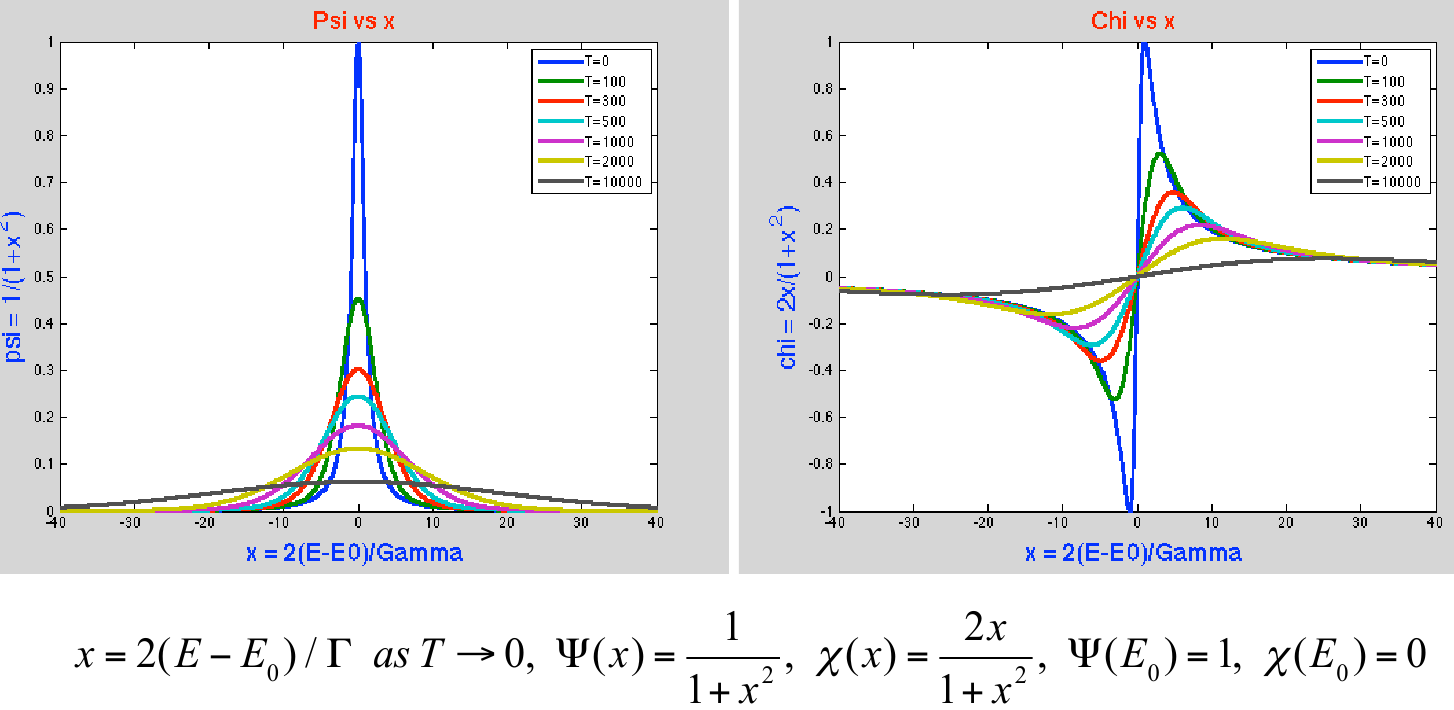
\includegraphics[width=4in]{images/r-m/psi-chi-plot.png}
  \caption{Plots of the Psi, Chi Functions} \label{psi-chi-plot} 
\end{figure}

Results: It is important to notice that \textit{all resonances contribute to all energies, even though their contributions can be infinitesimally}. 

\subtopic{Model For Unresolved Resonance Absorption}
We assume 25 eV resonance spacing, and assume
\begin{align}
\Gamma_{\gamma} &= 0.023 \eV \\
\Gamma_{n} &= 0.05 \sqrt{\frac{E}{E_{\mathrm{last}}}}  \eV
\end{align}
in which $E_{\mathrm{last}}$ means the last resonance energy used in the 14 resonance region. Notice that for the purpose of this excercise we assume this region to be unresolved, whereas in reality they are resolved. 


\end{document}
